\section{Pattern recognition algorithms}
\label{cha:Introduction}
\subsection{Introduction}
This section is devoted to presenting information about pattern recognition
algorithms. The main purpose is to describe algorithms that are used in this
thesis. 

Pattern recognition is a wide area of science in which we are interested in
assigning label from a given set of classes to every unknown pattern. The whole 
process of classification can be divided into few phases, where each has a
significant impact on the final classification accuracy:
\begin{enumerate}
    \item data collection,
    \item feature selection,
    \item model selection,
    \item classifier selection,
    \item training,
    \item testing.
\end{enumerate}
At first, few basic information and categories will be given 
about pattern classification task. Generally, the whole process
can be divided into two main categories:
\begin{itemize}
    \item unsupervised- objects (patterns) incoming to the system are not previously
        labeled and this is the system task to find an appropriate structure of
        the data, to establish the organization of the classes basing only on
        the available data; there is no statistical or expert knowledge at a
        hand,
    \item supervised- in this approach incoming patterns have labels and can
        be treated as a training set. A supervised learning algorithm analyzes the 
        training data and produces an inferred function, which is called a
        \textit{classifier}.
\end{itemize}
In this thesis supervised learning is considered because available datasets 
are labeled with class number. Another division is connected with the type and
structure of data:
\begin{itemize}
    \item statistical classification- attempts to classify objects
        based on a set of extracted features and available
        statistical model for the generation of these patterns. 
        Each pattern is represented in terms of $d$ features (measurements) 
        and is viewed as a point in $d$-dimensional feature space;
    \item syntactic or structural pattern recognition- assumes that pattern
        structure is quantifiable and extractable so that structural
        similarity of patterns can be assessed. It formulates hierarchical
        descriptions of complex patterns built up from simpler
        primitive elements. EKG waveforms, textured images and shape analysis 
        of contours are the examples of syntactic approach;
\end{itemize}

\subsection{Problem statement for pattern recognition task}
\label{cha:Problem_statement}
In this section the problem statement for the pattern
recognition algorithm will be presented. A supervised learning is assumed here which
means that each pattern is labelled by the label $j \in M$, where $M$ is an $m$-element set of
possible states numbered with the successive natural numbers. The state $j$ is
unknown and does not undergo the direct investigation. What can only be
measured are attributes or features by which a state manifests itself. For this
reason each object (pattern) is described by a $d$-dimensional measured feature vector $x \in
X$. In order to classify an unknown pattern classification algorithm uses knowledge stored in the training
set consisting of $N$ training patterns:
\begin{equation}
    S = (x_1, j_1), (x_2, j_2), \ldots, (x_N, j_N)
    \label{eq:training_pattern}
\end{equation}
In practice the decision algorithm with the learning phase should use knowledge included in the
training set $S$ so as the consequence the classifier has the following form:
\begin{equation}
    i=\Psi(S, x), \, i \in M
    \label{eq:decision_algorithm}
\end{equation}
In decision theory, to ensure that $\Psi$ approximates the problem as closely
as possible an additional loss function is introduced that assigns a specific
value to the loss resulting from producing an incorrect label. The particular loss
function depends on the type of label being predicted. In case of
classification problem it is usually zero-one loss function. This corresponds simply to
assigning a loss value of 1 to any incorrect labeling and is equivalent to computing
the accuracy of classification procedure over the set of training data.

\subsection{Rough sets}
\label{cha:Rough_set}
\subsubsection{Introduction}
\label{cha:Rough_set_introduction}
Rough sets theory represents the mathematical approach to deal with imperfect knowledge. 
In the standard pattern recognition task we need precise information about
pattern to recognize it, while rough sets can deal with vague or incomplete data. The problem of imperfect 
information has been tackled for a long time and it has become a crucial issue for many scientist.
One of the most prominent approaches in the recent years are fuzzy logic and rough sets.
In this section the latter approach is presented in greater details. 

Comparing with other methods, rough sets have many advantages, but one of the most important
one is its ability to works only on the raw data, with no additional assumption such 
as density probability in Bayesian algorithm \cite{bib38}, \cite{bib14}. The main facts about rough sets
algorithm can be summarized in few point presented below:
\begin{enumerate}
    \item simplifies data by the granulation pre-processing,
    \item is able to reduce attributes,
    \item generates set of easy to understand and readable decision
        \textit{IF-THEN} rules,
    \item evaluates significance of data.
\end{enumerate}

When talking about rough set theory one has to understand the concept of a set 
and how a rough set is related to the classical set represented in mathematic.
From the mathematical point of view the crisp (precise) set is a collection of 
objects of interest and is uniquely determined by its elements. In other words,
it means that every element must be uniquely classified as belonging to the set 
or not (true or false). For example, the set of odd numbers is crisp because every
number is either odd or even and can not be partially in both. 

This is the pure theory, but generally problems form the nature are much more
complicated and require more complex decisions than whether an objects belong to
the set or not, because for some phenomenon we can not precisely describe element
membership. Consider the group of people and division into the set of small and
high people. The height is not a precise but a vague concept and data vagueness can 
be met in many problems from the nature. Here is the spot for rough sets
theory where the vagueness is expressed by a boundary region of a set. 

\subsubsection{Basic notation}
\label{cha:Rough_set_basic_notation}
Rough sets theory can be described in many ways and notations. In this paper
the approach presented in \cite{bib49} is applied. 

In rough sets theory to represent datasets (information) we introduce a notion 
called an \textit{information system} \cite{bib37}, \cite{bib39}. 
It can be described by 4-tuple
\begin{equation}
    IS = <U, Q, V, f >
    \label{eq:information_system}
\end{equation}
where the notation used in eq. (\ref{eq:information_system}) is as follows:
\begin{itemize}
    \item $U$ is the universe of discourse  which is a finite set of objects
        (patterns),
    \item $Q$ is a finite set of attribute by  which each patterns manifests
        itself (is described),
    \item $V = \bigcup V_q$, $V_q$ represents a domain of attribute $q$,
    \item $f:U \times Q \rightarrow V$ is a total information function, such that
        $\bigvee_{q\in Q, x \in U} f(x,q) \in U$,
\end{itemize} 
The information system can be represented as a finite table in which 
columns are labeled by attributes and each rows stands for an object from
$IS$. Over the information table we can define decision table
$T$ where the set of attributes $Q$ is disjoined into two
subset $C$ and $D$. The set $C$ is a subset of 
condition attributes, and the set $D$ contains decision attributes 
by which we can partition set $U$ into decision classes.

From the granular nature of rough sets it may happen that some objects 
in the $U$ are indistinguishable due to the limited information caused by
granulation process. Taking this into account let define an indiscernibility
relation $R \rightarrow U \times U$, representing the 
lack of knowledge about patterns in the set $U$. The indiscernibility relation on
$U$ can be extended and associated with every non-empty subset of attributes $P \subseteq Q$
and is defined by eq. (\ref{eq:indiscernibility})
\begin{equation} 
    I_P = \{ (x, y) \in U \times U: f(x, q) = f(y,q), \bigvee_{q \in P}\}
    \label{eq:indiscernibility}
\end{equation}
Now having $I_P$ we can say that objects $x$ and
$y$ are $P$-indiscernible by a set of attributes $P$ if $y \, I_P \, x$. Relation
$I_P$ divides the set $U$ into blocks (concepts) of $P$-indiscernible objects.
The $P$-elementary set containing objects $P$-indiscernible with $x \in U$ is
referred as $I_P(x)$ and defined as follows:
\begin{equation} 
    I_P = \left\{ y \in U: y \, I_P \, x \right\}
    \label{eq:p_indiscernible}
\end{equation}

By representing a target concept $X$ as a subset of $U$ we would like to
describe it with respect to $R$. Additionally let assume that $P$ is a non-empty
subset of attributes from $Q$. In rough sets reasoning an object membership to a
set can be represented in two ways:
\begin{enumerate}
    \item an object $ x \in U$ certainly belongs to $X$ if
        all objects from the $P$-elementary set defined by $I_P(x)$ also belong to $X$.
        A set of all objects certainly belonging to $X$ creates the $P$-lower
        approximation of $X$ and can be represented as follows:
        \begin{equation}
            \underline{I_P} = \{ x \in U: I_P(x) \subseteq X\}
            \label{eq:lower_approximation}
        \end{equation}
    \item an object $x \in U$ can possibly belong to $X$ if at least one object
        from $P$-elementary set $I_P(x)$ can possibly belong to $X$. All the
        objects that could possibly belong to $X$ are denoted as $P$-upper
        approximation of $X$, defined as:
        \begin{equation}
            \overline{I_P} = \{x\in U: I_P(x) \, \cap \, X \neq \emptyset \}
            \label{eq:upper_approximation}
        \end{equation}
        Therefore the set $U - \overline{I_P}$ represents the negative region
        containing the set of objects that can be definitely ruled out as
        members of the target set $X$.
\end{enumerate}

The tuple $<\underline{I_P}, \overline{I_P}>$ representing a lower boundary of
the target $X$ and the upper boundary of the target $X$ creates a rough set \cite{bib34}.
Using above notion we can define $P$-boundary region which is a difference
between upper and lower approximation \cite{bib14}. 
\begin{equation}
    BN_P(X) = \overline{I_P} - \underline{I_P}
    \label{eq:boundary_region}
\end{equation}
The $BN_P(X)$ is a set of elements which can not be certainly classified neither
as $X$ nor as not-$X$ with respect to the set of attributes $P$. If the
boundary region of $X$ is empty then the set represented by tuple
$<\underline{I_P}, \overline{I_P}>$ 
is crisp, otherwise we deal with inexact set which is called rough set. 
Until this moment we can see that rough sets concept can be defined quite generally by means of topological
operations: interior and closure, called approximations. They express the
knowledge about pattern in terms of granules, not by a precise measure
\cite{bib40}.

The illustrative example of rough sets reasoning is presented in fig. \ref{fig:rough_set_example}
\begin{figure}[H] 
    \begin{center}
        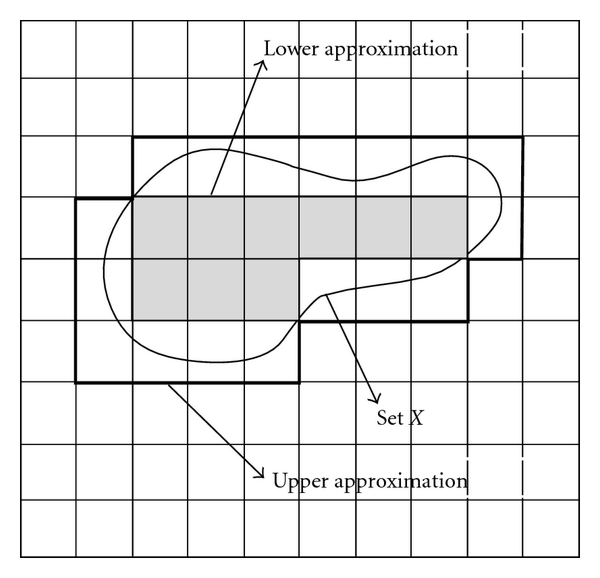
\includegraphics{fig/rough_set.png}
    \end{center}
    \caption{Rough sets example presenting lower and upper approximations}
    \label{fig:rough_set_example}
\end{figure}

\subsubsection{Rough sets indicators}
\label{cha:Rough_sets_indicators}
In rough sets theory we can define few indicators to measure the quality of
approximation. First of all with every 
subset of $X \subseteq U$ described by $P$ subset of attributes we can 
associate an indicator called an accuracy of approximation defined as:
\begin{equation}
    \alpha_P(X)=\frac{\underline{I_P}(X)}{\overline{I_P}(X)}
    \label{eq:accuracy_approximation}
\end{equation}
The graeter $\alpha_P(X)$ is the better approximation we have which means that
many objects can be certainly classified as belonging to the target set $X$.

Another important indicator is a quality of approximation of $X \subseteq U$ by
attributes from subset $P$. It represents the percentage of correctly classified 
objects using attributes $P$ from subset $X$:
\begin{equation}
    \gamma_P(X) = \frac{\overline{I_P}(X)}{|X|}
    \label{eq:quality_approximation}
\end{equation}
Assuming that we can partition $U$ into $n$ decision classes using $P$
non-empty subset of attributes from $C$, the quality of classification can be
defined as the ration of all correctly classified objects into classes:
\begin{equation}
    \gamma_P(CLASS) = \frac{\sum_{i=1}^{n}\overline{I_P}(CL_i)}{|U|}
    \label{eq:class_quality}
\end{equation}

These indicators can be used in determining the quality of rough set algorithm
or for finding the optimal reduct. Generally, the main goal in constructing
rough sets algorithm is to obtain rule set with possible the greatest number of
certain decisions.

\subsubsection{Properties of rough sets}
Similarly to classical sets, rough sets can be described by the
following properties:
\begin{enumerate}
    \item $\overline{I_P} \subseteq \, X \, \subseteq \, \underline{I_P}$
    \item $\overline{I_P}(\emptyset) = \underline{I_P}(\emptyset) = \emptyset;
        \; \overline{I_P}(U) = \underline{I_P}(U) = U $
    \item $\overline{I_P}(X \cup Y) = \overline{I_P}(X) \cup \overline{I_P}(Y)$
    \item $\underline{I_P}(X \cap Y) = \underline{I_P}(X) \cap \underline{I_P}(Y)$
    \item $\overline{I_P}(U-X) = -\underline{I_P}(X)$
    \item $\underline{I_P}(U-X) = -\overline{I_P}(X)$
\end{enumerate}
It is easily seen that the lower and the upper 
approximations of a set are interior and 
closure operations in a topology generated by the 
indiscernibility relation $I_P(X)$. Additionally, in rough sets theory 
we can define four types of data vagueness \cite{bib40}:
\begin{itemize}
    \item $\overline{I_P}(X) \neq \emptyset,\, \underline{I_P}(X) \neq
        \emptyset$ $IF\; X$ is roughly $I_P$-definable. It means that using $I_P$ for some
        elements from $U$ we can decide whether they belong to $X$ or $U-X$;
        
    \item $\overline{I_P}(X) \neq \emptyset,\, \underline{I_P}(X) \neq U$ $IF\;
        X$ is internally $I_P$-indefinable. It means that using $I_P$ we are able to decide
        which elements from $U$ belong to $U-X$, but we don't know if they
        belong to $X$;
    \item $\overline{I_P}(X) \neq \emptyset,\, \overline{I_P}(X) = U$ $IF\;
        X$ is externally $I_P$-definable. It means that using $I_P$ we are able to decide
        which elements from $U$ belong to $X$, but we don't know if they belong
        to $U-X$;
    \item $\overline{I_P}(X) \neq \emptyset,\, \overline{I_P}(X) = U$ $IF\;
        X$ is totally $I_P$-indefinable. It means that using $I_P$ we are unable to decide
        for any element from $U$ if it belongs to $X$ or $-X$;
\end{itemize}
\subsubsection{Rough sets reasoning from data}
The category description can be done in two ways:
\begin{enumerate}
    \item extensional,
    \item intentional.
\end{enumerate}
Each of these approaches define how pattern from dataset is
described and assigned to the proper class. To correclty represent 
a target concept (class we try to recognize from all objects) from dataset an
algorithm should be able to identify all objects belonging 
to this category. With the first method presented above (extensional), we have no insight 
into decision engine so we do not know how to assign new objects to the category.
In the second approach the particular category is described by the set of rules. 
The same method is applied in rough sets algorithm where elementary 
granules (concepts) of knowledge build blocks consisting 
of indiscernible patterns from the universe of discourse $U$. 

As stated in section \ref{cha:Rough_set_basic_notation} considered dataset or
problem can be represented as a table. When decision attributes from $D$ are
added to this table it becomes a decision table $T$ where each
row is associated with decision rule. Below, the practical example is presented to 
clear all the things out. 

Let consider the well-known problem of patients suffering from
flu \cite{bib39}, \cite{bib40}. The task is to decide if a patient described by
3 attributes is ill or not. Table \ref{tab:example_rough_set} 
represents an information system $IS$ about healthy patient and those suffering
from flu. Attributes: \textit{Headache}, \textit{Muscle-pain},
\textit{Temperature} are called condition attributes and are denoted as ($c_i,i \in (1, \ldots, q)$),
while the attribute \textit{Flu} (last column in table
\ref{tab:example_rough_set}) is chosen as a decision attribute $c_d$.
\begin{table}[H] 
    \centering
    \caption{Example dataset showing healthy patients and suffering from flu}
    \begin{tabular}{|c|c|c|c|c|c|}
        \hline 
    Patient & Headache $c_1$& Muscle pain $c_2$& Temperature $c_3$& Flu $c_d$\\ \hline \hline
    p1 & no & yes & high & yes \\ \hline
    p2 & yes & no & high & yes \\ \hline
    p3 & yes & yes & very high & yes \\ \hline
    p4 & no & yes & normal & no \\ \hline
    p5 & yes & no & high & no \\ \hline
    p6 & no & yes & very high & yes \\ \hline    
    \end{tabular}
    \label{tab:example_rough_set}
\end{table}

Each row of a decision table determines a decision rule. 

\begin{tabular}[H]{l}
    Rule 1:  IF $c_1$ IS 'NO' AND $c_2$ IS 'YES' AND $c_3$ IS 'HIGH' THEN $c_d$
    IS 'YES' \\
    Rule 2:  IF $c_1$ IS 'YES' AND $c_2$ IS 'NO' AND $c_3$ IS 'HIGH' THEN $c_d$
    IS 'YES' \\
    Rule 3:  IF $c_1$ IS 'YES' AND $c_2$ IS 'YES' AND $c_3$ IS 'VERY HIGH' THEN
    $c_d$ IS 'YES' \\
    Rule 4:  IF $c_1$ IS 'NO' AND $c_2$ IS 'YES' AND $c_3$ IS 'NORMAL' THEN
    $c_d$ IS 'NO' \\
    Rule 5:  IF $c_1$ IS 'YES' AND $c_2$ IS 'NO' AND $c_3$ IS 'HIGH' THEN $c_d$
    IS 'NO' \\
    Rule 6:  IF $c_1$ IS 'NO' AND $c_2$ YES 'NO' AND $c_3$ IS 'VERY HIGH' THEN
    $c_d$ IS 'YES'  
\end{tabular}


Analyzing table \ref{tab:example_rough_set}, it is noticeable that some
patients can not be distinguished between each other.
It is possible to generate different indiscernible relations based on 
the chosen attributes. In case of \textit{Headache} attribute patients: $p2$,
$p3$, $p5$ are indiscernible; patients $p2$, $p5$ are
indiscernible with respect to attributes \textit{Headache},
\textit{Muscle-pain} and \textit{Temperature}, or if we use \textit{Headache}
and \textit{Muscle-Pain} the set $U$ can be divided into three sets:
\{$p1$, $p4$, $p6$\}, \{$p2$, $p5$\}, \{$p3$\}.

Now it is time for defining key features of rough sets. Over the table
\ref{tab:example_rough_set} we can choose two concepts (target sets):
\textit{Flu} and \textit{Not Flu}. For the first concept the lower approximation
set of patient certainly having flu is \{$p1$, $p3$, $p6$\}, while the upper
approximation of patients possibly suffering from flu is \{$p1$, $p2$, $p3$,
$p5$, $p6$\}. The boundary region for concept \textit{Flu} is a set of \{$p2$, $p5$\} 
patients. For the concept \textit{Not Flu} the lower approximation is the set
\{$p4$\}, the upper approximation is the set \{$p2$, $p4$, $p5$\}, whereas the 
boundary region is again the set \{$p2$, $p5$\}.

Additionally, we can measure the accuracy of approximation $\alpha_P(x)$ for each concept.
This can indicate if the set of attributes used for describing the concepts is correctly
chosen. For the \textit{Flu} concept where $X$=\{$p1$, $p2$, $p3$, $p6$\}
(those patterns where the decision attribute is \textit{Yes}) is described by
set of attributes $P$=\{\textit{Headache}, \textit{Muscle-pain},
\textit{Temperature}\} the accuracy of approximation is:
$$\alpha_P(Flu) = \frac{|\{p1, p3, p6\}|}{|\{p1, p2, p3, p5, p6\}|} = \frac{3}{5}$$
On the other hand, when we take only one attribute
$P$=\{\textit{Temperature}\}, then for the concept \textit{Flu} we get the lower approximation of 
as a set of \{$p3$, $p6$\} and the upper approximation of \{$p1$, $p2$, $p3$,
$p5$, $p6$ \}. In this case the accuracy of approximation is as follows:
$$\alpha_P(Flu) = \frac{2}{5}$$
To sum up, $\alpha_P(x)$ is a very important indicator in
rough sets theory and tells which attributes better characterize target
concept. This example has shown that because of the granule representation of
knowledge in rough sets approach some object can not be discerned. It is very
important to choose proper condition attributes because they determine how
upper and lower approximations are represented by objects from $U$. 


\subsection{Fuzzy logic}
\label{cha:Fuzzy_logic}
\subsubsection{Introduction}
In fuzzy logic an element membership to a set is described by a membership function 
which assigns value from interval $[0, 1]$:
\begin{equation}
    \mu_A(x):U\rightarrow [0,1], \, A \subseteq U, \, x \in A
    \label{eq:fuzzy_function}
\end{equation}
The properties of membership function $\mu$ are as follows:
\begin{itemize}
    \item $\mu_{\emptyset}(x) = 0, \, x \in U$
    \item  $\mu_{U}(x) = 1, \, x \in U$
    \item  $\mu_{X}(x) \leq \mu_{Y}(x), \, IF X \subseteq Y$
    \item  $\mu_{\overline{A}}(x) = 1 - \mu_{A}(x), \, x \in U$
\end{itemize}
where $\emptyset$ is an empty set and $\overline{A}$ is the complement of the
set $A$.

Fuzzy logic is a superset of Boolean logic that 
has been extended to handle the concept of partial truth - values between ``completely 
true'' and ``completely false'' \cite{bib6}, \cite{bib12}. This theory was introduced by 
Dr. Lotfi Zadeh in the 1960's as a tool for modeling the uncertainty of natural language. 
This approach can be applied to many problems, here analyze only few examples:
\begin{itemize}
    \item days of a week- there is a question which day is mostly associated
        with a weekend. Generally, we would assume that the membership value
        $g$ associated with each day will be as follows:
        \{Monday=0, Tuesday=0.2, Wednesday=0.4, Thursday=0.5, Friday=0.7,
        Saturday=1.0, Sunday=0.9\};
    \item the seasons- there is not evident boundary when one season stops and
        another starts. This example can be illustrated quite precisely by fig.
        \ref{fig:seasons};
        \begin{figure}[H]
            \begin{center}
                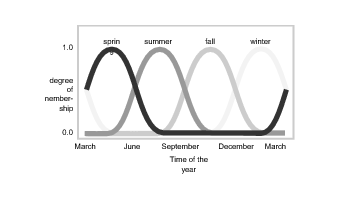
\includegraphics{fig/seasons.png}
            \end{center}
            \caption{Example of how fuzzy logic can be used to describe the
            seasons of the year\footnotemark}
            \label{fig:seasons}
        \end{figure}
        \footnotetext{source: http://www.mathworks.com/help/toolbox/fuzzy/bp78l6_-1.html}
    \item the height (small and tall definitions)- from the group of people it
        is hard to define who is tall and who is small interchangeably. To
        solve this problem we can define the concept \textit{Tall} and assign
        value to each person describing its height. This process is presented in
        fig. \ref{fig:fuzzy_tall};
        \begin{figure}[H]
            \begin{center}
                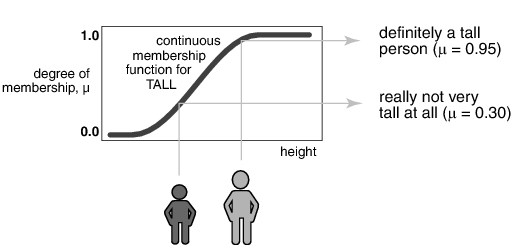
\includegraphics{fig/fuzzy_tall.png}
            \end{center}
            \caption{Fuzzy approach for defining person height\footnotemark}
            \label{fig:fuzzy_tall}
        \end{figure}
        \footnotetext{source: http://www.mathworks.com/help/toolbox/fuzzy/bp78l6_-1.html}
\end{itemize}

Similarly to the section \ref{cha:Rough_set_introduction}, let consider more deeply the problem of defining 
if person is small or tall in the group of people. First of all, we have to define a fuzzy
set (concept) \textit{Tall} which will answer the question 
"to what degree is person $x$ tall?". Zadeh describes \textit{Tall} as a
linguistic variable, which represents our cognitive category of "tallness"
\cite{bib25}. The procedure is as follows: to each person in the group 
assign a degree of membership (value from $[0, 1]$ range) in the fuzzy subset \textit{Tall}
based on the membership function (for example the same as presented in fig.
\ref{fig:fuzzy_tall}). Table \ref{tab:fuzzy_logic_example} shows the degree of
membership how person is tall in the group of six people.
\begin{table}[H]
    \centering
    \caption{Table describing how person is tall by the fuzzy logic linguistic
    variable}
    \begin{tabular}{|c|c|c|}
        \hline
        Person & Height [m] & degree of tallness \\ \hline \hline
        p1 & 1.5 & 0.00 \\ \hline
        p2 & 1.6 & 0.21 \\ \hline
        p3 & 1.7 & 0.44 \\ \hline
        p4 & 1.8 & 0.52 \\ \hline
        p5 & 1.9 & 0.69 \\ \hline
        p6 & 2.0 & 1.00 \\ \hline
    \end{tabular}
    \label{tab:fuzzy_logic_example}
\end{table}

Fuzzy numbers are fuzzy subsets generated over the attribute domain. 
They have a peak or plateau with membership grade 1 over which the 
members of the universe are completely in the set.  The membership 
function is increasing towards the peak and decreasing away from it. 
There are different types of membership functions and their usage 
strongly depends on the type of considered problem. One of the most 
commonly used in the literature are: triangular, trapezoidal, Gaussian shapes
(see example in fig. \ref{fig:fuzzy_example_1}).

\subsubsection{Fuzzy reasoning from data }
Reasoning in fuzzy logic is based on decision rules, the same as in rough sets
approach \cite{bib11}. 
Rules are expressed in the form of IF \textit{CONDITIONS} THEN \textit{DECISION}
where \textit{CONDITIONS} can be divided into antecedent set ($A_{ri}, \, i \in
(1, \ldots, q)$) and \textit{DECISION} is the consequent determining the
output of the rule. In the pattern recognition task when we deal with patterns
described by $d$ features then decision rules have the form presented by eq. (\ref{eq:rule_example})
\begin{equation}
    IF\, x_1=A_{r1}\, AND\, x_2=A_{r2}\, AND\, \ldots\, AND\, x_d=A_{rd}\, THEN\,
class\, C_r\, with \, CF_r
    \label{eq:rule_example}
\end{equation}

The \textit{AND}, \textit{OR}, and \textit{NOT} operators of 
Boolean logic exist in fuzzy logic and are usually defined it two ways:
\begin{itemize}
    \item the minimum, maximum, and complement operator from the set. 
        When they are defined this way, they are called the Zadeh operators
        \cite{bib2};
    \item multiplication, addition and subtraction from one. In this case
        normalization procedure is needed because after these operation the
        final result can be grater than one;
\end{itemize}
Fuzzy logic classification is based on three main steps:
\begin{enumerate}
    \item fuzzyfication- in the fuzzyfication process we  
        convert continuous quantity into fuzzy number based on the appropriate
        membership function value. It requires defining
        membership grade of crisp input $x$ in the fuzzy set;
    \item rule induction- there are different types of fuzzy inference systems,
        but one of the most commonly used (the same as in this paper) is
        Mamdani inference system \cite{bib46}, another method is Sugeno-Type
        Fuzzy Inference;
    \item deffuzification- the process of producing a quantifiable (crisp) result
        from available fuzzy sets and corresponding membership degrees;
\end{enumerate}
The whole process of fuzzy reasoning is presented in fig.
\ref{fig:fuzzy_reasoning}
\begin{figure}[H]
    \begin{center}
        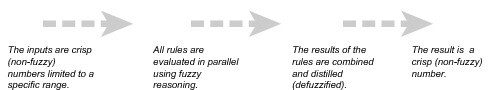
\includegraphics[width=\textwidth]{fig/fuzzy_steps.png}
    \end{center}
    \caption{Steps applied in fuzzy reasoning.\footnotemark}}
    \label{fig:fuzzy_reasoning}
\end{figure}
\footnotetext{source: http://www.mathworks.com/help/toolbox/fuzzy/bp78l6_-1.html}

Let consider a simple example, which should clear all ambiguities (the following 
example is based on \cite{bib0}). The problem is connected with estimating the
level of the risk involved in software engineering project. There are two
inputs to the system (funding, staffing) and one output
(risk). Membership functions are represented as of triangular shapes (fig. \ref{fig:fuzzy_example_1}) 
\begin{figure}[H]
    \begin{center}
        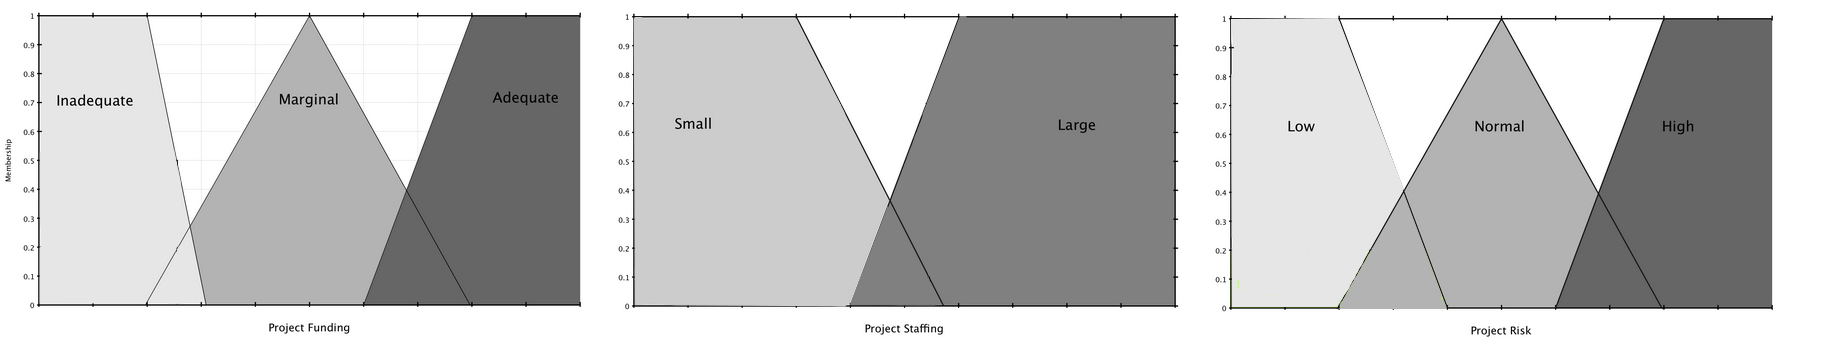
\includegraphics[width=\textwidth]{fig/fuzzy_example_1.png}
    \end{center}
    \caption{Input and output fuzzy linguistic variables for the described
    system.}
    \label{fig:fuzzy_example_1}
\end{figure}
The next important thing in fuzzy logic beside fuzzy values are fuzzy rules. In
this problem they are provide a priori and are as follows:
\begin{table}[H]
    Rule 1: IF funding IS adequate OR funding IS small THEN risk IS
    low \\
    Rule 2: IF funding IS marginal AND staffing IS large THEN risk IS
    normal \\
    Rule 3: IF funding IS inadequate THEN risk IS high
\end{table}
Let say that we want to calculate project risk for inputs: funding~$=35$ and
staffing~$=60$. 
\begin{enumerate}
    \item The first step is to convert crisp values into fuzzy representation.
        After activating each input membership functions the fuzzy values are as follows:
        $$
            \begin{array}[H]{l}
                input \;1 \\ \hline
                \mu_{inadequate}(35) = 0.5 \\
                \mu_{marginal}(35) = 0.2 \\
                \mu_{adequate}(35) = 0.0 \\ \\
                input \;2 \\ \hline
                \mu_{small}(60) = 0.1 \\
                \mu_{large}(60) = 0.7 \\ 
            \end{array}
        $$
    \item Now it is  time for rule induction where OR is treated as a summation, AND
        as multiplication operator. 
        $$
            \begin{array}[H]{ll}
                Rule \,1: & \mu_{low} = 0.0 + 0.1 = 0.1 \\
                Rule \,2: & \mu_{normal} = 0.2 \cdot 0.7 = 0.14 \\
                Rule \,3: & \mu_{high} = 0.5 \\
            \end{array}
        $$
    \item After performing clipping of consequent membership functions for each
        rule (example given in fig. \ref{fig:fuzzy_centroid}), the final crisp output can be calculated. It is done by
        defuzzification method, where one of the most commonly used is a centroid
        formula given by eq. (\ref{eq:fuzzy_centroid}) \cite{bib0}, \cite{bib1}.
        \begin{equation}
            CO = \frac{\sum\nolimits_{x=a}^{b}\mu_A(\chi)\cdot
            x}{\sum\nolimit_{x=a}^{b}\mu_A(\chi)}
            \label{eq:fuzzy_centroid}
        \end{equation}
        \begin{figure}[H]
            \begin{center}
                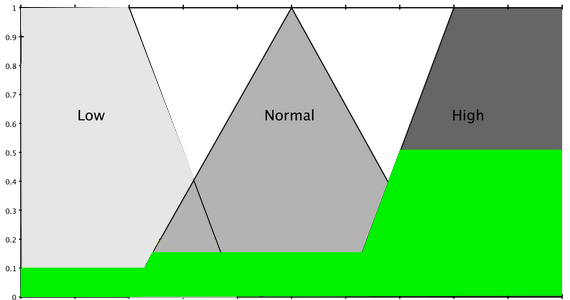
\includegraphics[width=0.6\textwidth, height=0.4\textwidth]{fig/fuzzy_centroid.png}
            \end{center}
            \caption{Example of clipping the consequent membership function
            as the result of rule induction}
            \label{fig:fuzzy_centroid}
        \end{figure}
        Using eq. (\ref{eq:fuzzy_centroid}) the output of the system is as follows:
        $$
        CO = \frac{(0+10+20)\cdot 0.1 + (30+40+50+60)\cdot 0.14 + (70 + 80 + 90
        + 100)\cdot 0.5}{0.1\cdot 3 + 0.14\cdot 4 + 0.5\cdot 4 } = 69.3
        $$
    It means that for input values funding~$=35$ and staffing~$=60$ the project
    risk is about $69\%$.
\end{enumerate}
\subsubsection{Genetic-based machine learning approaches}
In the literature one can find many examples of fuzzy logic
applications for pattern recognition task \cite{bib3}, \cite{bib9}.
Generally, there are two main approaches:
\begin{enumerate}
    \item some expert knowledge is available and fuzzy rules are created
        beforehand,
    \item no knowledge about data set is present so some techniques of data
        mining must be applied to extract rules from the training set.
\end{enumerate}
At this point it must be strongly emphasized that in this thesis the main focus is based on
fuzzy algorithm for pattern recognition task where there is no prior knowledge 
about fuzzy system and decision rules. There are different approaches for
construction fuzzy logic algorithm from raw dataset, for example optimization techniques
such as gradient descent or heuristic algorithms \cite{bib8}, \cite{bib16},
\cite{bib28}. In this paper the genetic algorithm
is proposed for creating an optimal rule set. 

One can wonder what is the purpose of applying genetic algorithm into rule
generation. For the simplicity let consider such a case where $N$ training
patterns are available and nothing more. Now the following question arises: 
how to properly divide the feature space into fuzzy set, and how to generate
decision rules when there is no expert knowledge. The simplest and
straightforward solution is to create let say 10 triangular membership functions for each
attribute, and check each possible combination. Is this approach optimal? The
efficiency of this solution strongly depends on the complexity of the problem.
For $d$-dimensional feature space and $k$ fuzzy membership functions per each attribute
the number of possible combination for generating one rule is equal to $k^d$.
For greater $d$ (for example wine dataset from \textit{UCI} repository has 13
attributes) it is impossible to find the proper rule combination in a reasonable
time. Here is an open spot for genetic algorithm to show its searching
abilities.

There are two main methods of genetic-based machine learning approaches
\cite{bib30}, \cite{bib31}:
\begin{enumerate}
    \item Michigan template- it is a population of fuzzy rules and a single
        fuzzy rule is handled as an individual (see fig. \ref{fig:michigan}). 
        The evaluation of each fuzzy rule is performed by classifying all the 
        given training patterns by the available rule set $N_{rule}$. At the 
        end of each iteration new individuals are created through genetic operators 
        and merged to the current population. For the next generation $N_{rule}$ 
        best individuals are taken. The whole procedure can be summarized as follows:
        \begin{enumerate}
            \item generate $N_{rule}$ fuzzy rules,
            \item evaluate the fitness of each fuzzy rule in the current
                population,
            \item generate $N_{replace}$ fuzzy rules using genetic operators,
            \item merge $N_{replac e}$ fuzzy rules with current population and
               choose the best $N_{rule}$ individuals for the next generation,
             \item return to point  $(b)$ is stopping condition is not fulfilled
                (number of generations).
        \end{enumerate}
        \begin{figure}[H]
            \begin{center}
                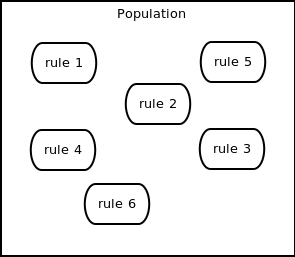
\includegraphics[width=0.5\textwidth, height=0.4\textwidth]{fig/michigan.png}
            \end{center}
            \caption{Example of Michigan approach for constructing Genetic Fuzzy logic algorithm}
            \label{fig:michigan}
        \end{figure}
    \item Pittsburgh template- in this approach a set of fuzzy rules is handled
        as an individual (see fig. \ref{fig:p}). In this case the length of a single individual is
        equal to $n\cdot N_{rule}$, where $n$ is the length of single fuzzy rule.
        Algorithm starts with $N_{pop}$ randomly generated rule sets. The
        fitness value of a single individual is the number of correctly
        classified patterns in the training set by a given rule set.
        The procedure for this algorithm is as follows:
        \begin{enumerate}
            \item generate $N_{pop}$ individuals consisting of $N_{rule}$ fuzzy
                rules each,
            \item calculate the fitness value of each rule set (individual)
                using training dataset,
            \item generate $N_{replace}$ new rule set using genetic operators,
            \item merge $N_{replace}$ fuzzy rule sets  with current population and
                choose the best $N_{pop}$ individuals for the next generation,
            \item return to point $(b)$ is stopping condition is not fulfilled
                (number of generations).
        \end{enumerate}
        \begin{figure}[H]
            \begin{center}
                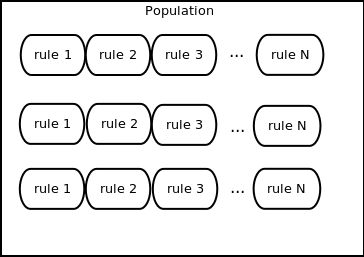
\includegraphics[width=0.5\textwidth, height=0.4\textwidth]{fig/pittsburgh.png}
            \end{center}
            \caption{Example of Pittsburgh approach for constructing Genetic Fuzzy logic algorithm}
            \label{fig:p}
        \end{figure}
\end{enumerate}
In this thesis the first approach is implemented in simulations which means that
individual is modeled as a single rule. 

\subsection{Attribute selection}
\label{cha:Attribute_reduction}
Many problem are complex and multidimensional. For example Sonar dataset from
\textit{UCI} Repository has 60 attributes describing a single pattern. 
Usually we hope to recognize pattern in a relatively
lower dimension to reduce the cost in measuring and processing information and
enhance the interpretability of learned models. Feature selection or reduction 
is done for classifiers to remove the noise and superfluous data. Generally,
this is not an easy task and requires a lot of computation \cite{bib1}, \cite{bib5}.  

A reduct is a set of attributes that ensures the same classification of
elements from $U$ as the rudimentary set of attributes. More than one reduct
can exist for one information system, but there is only one core reduct in $Q$.
The core reduct is the set of attributes from $Q$ that all the 
attributes are indispensable. It means that we cannot remove those features
from the set because we will loose information about patterns. 

An attribute is dispensable if the following criterion is fulfilled:
$$I(P) = I(P-{a}), \, \textrm{for} \, \{a\} \in P \subseteq  Q $$

In the literature there are many examples of how to apply attribute selection:
\begin{itemize}
    \item information measures,
    \item distance measures,
    \item dependence measures,
    \item consistency measures.
\end{itemize}
Different approaches provide various results and their application strictly
depends on the type of data. One of the best known methods are: Principal
Component Analysis, Factor analysis or optimization and heuristic techniques.
In the recent years heuristic methods are very often used because of their
speed and searching abilities. A lot of work has been devoted to feature
extraction and this aspect in not the main goal of this research.
Basing on the results and conclusions presented in the literature, in this thesis a 
genetic algorithm is proposed for extracting valuable features from the set of 
all attributes \cite{bib27}, \cite{bib48}.

\subsection{Genetic algorithm}
\label{cha:Genetic_algorithm}
Genetic Algorithm is an element of evolutionary computation, which is a 
rapidly growing area of soft computing \cite{bib42}, \cite{bib43}. GA is based on the principles of
natural selection and genetic modification. As optimization methods, GA 
operates on a population of points, designated as individuals. Each 
individual of the population represents a possible solution of the 
optimization problem. Individuals are evaluated depending upon their 
fitness which indicates how well an individual of the population solves 
the optimization problem. To sum up, GA has the following general features:
\begin{enumerate}
    \item GA operates with a population of possible solutions (individuals) 
        instead of a single individual. Thus, the searching process can be 
        carried out in a parallel form or sequentially;
    \item GA is able to find the optimal or sub-optimal solutions in complex
        and large search spaces. Moreover, it can be applied to nonlinear 
        optimization problems with constraints defined in discrete or continuous 
        search spaces;
    \item GA examines many possible solutions at the same time, so there is a 
        higher probability that the search process can converge to an optimal
        solution;
\end{enumerate}
There are four main parts in each GA process to consider (graphically
presented as a flow chart \ref{fig:genetic_scheme}):
\begin{enumerate}
    \item the problem representation or encoding,
    \item fitness or objective function definition,
    \item fitness-based selection,
    \item evolutionary reproduction of candidate solutions (individuals or
        chromosomes).
\end{enumerate}
\begin{figure}[H] 
    \begin{center}
        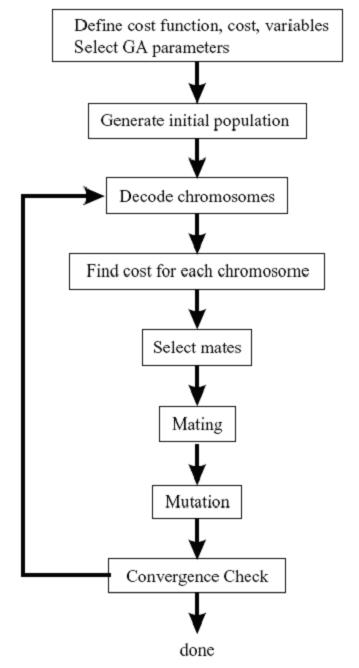
\includegraphics[height=0.5\textwidth]{fig/genetic.png}
    \end{center}
    \caption{Diagram representing phases in genetic algorithm evaluation}
    \label{fig:genetic_scheme}
\end{figure}

Genetic algorithms are widely used as a search techniques in the various fields. 
In this thesis it will be used for finding an optimal cuts in the attribute
space for rough sets algorithm and for obtaining optimal decision rule set in
fuzzy logic algorithm. The success of a genetic algorithm can be quantified by estimating 
the cost and the quality of final obtained solution. 

In the literature there can be found many examples of how GA is useful in solving hard 
optimizations problems, but beside unquestionable advantages there also exist downsides. 
A traditional GA without any diversity maintenance mechanism often suffers from getting 
stuck on the suboptimal peaks, because almost the entire GA population would have converged 
to a single peak, as a result of the rapid loss of population diversity \cite{bib44}, \cite{bib45}. 

There is a great deal of work showing how to set the optimal parameters in an evolutionary 
algorithm to obtain required speedup and solution accuracy, but this is not the main issue 
in this thesis. For more exact information see \cite{bib42}, \cite{bib43}.

When designing genetic algorithm one of the most important thing is to ensure proper crossover 
and mutation operations. More precise information about these operators will be
presented in section \ref{cha:Algorithm_construction}.

\subsection{Hybrid classifiers} 
\label{cha:Hybrid_classifiers}
In the recent years there is an increasing interest in methods of combining
multiple learning systems into hybrid one \cite{bib5}, \cite{bib6}. The main advantage of such approach
is its ability to find different relations and  explanation for the dataset for each
classifier. If classifiers make errors on different parts of the feature space
or apply different reasoning it is possible that the ensemble of classifiers will complement each other and
the final classification will be better. 

Generally, there are two types of hybrid classifiers (example presented in fig.
\ref{fig:hybrid}):
\begin{enumerate}
    \item multiexpert systems- classifiers work in parallel, each of them is
        trained and tested on the same data and independent decisions are
        combined to compute the final result. The most common example is a
        majority voting;
    \item multistage systems- classifiers are connected in a sequence where the
        next classifier is trained and used for classification only if the
        previous classifier rejected the pattern;
\end{enumerate}
It is hard to decide which approach is better. Each system has its pros
and cons and the choice depends of the type of dataset and available
classifiers. In this thesis the second approach is implemented where the first
segment is built as rough sets classifier and the second one is constructed
using fuzzy logic.
\begin{figure}[H]  
    \begin{center}
        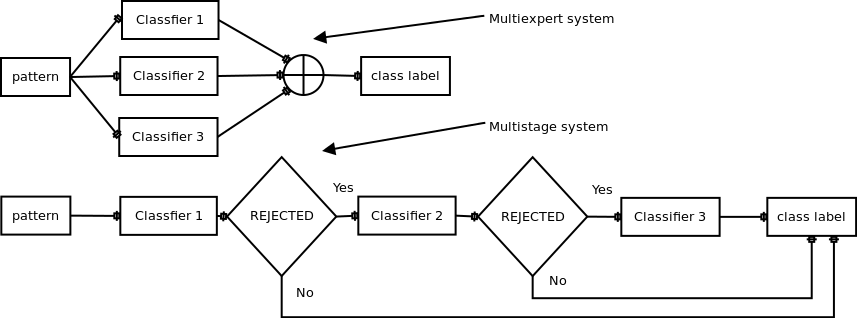
\includegraphics[width=\textwidth]{fig/hybrid.png}
    \end{center}
    \caption{Example of two approaches for constructing hybrid classifiers}
    \label{fig:hybrid}
\end{figure}
